\documentclass{beamer}
\usepackage[utf8]{inputenc}
\usepackage[english]{babel}

% -- Including some standard packages --
\usepackage{graphicx}
\usepackage{soul}
\usepackage{hyperref}
\usepackage{colortbl}
\usepackage{dsfont}
\usepackage{soul}

% -- Choosing theme --

\usetheme{Boadilla}
\usecolortheme{whale}
\setbeamercolor{alerted text}{fg=purple} % Making alerted text non-red

% Tikz
\usepackage{tikz}
\usetikzlibrary{matrix,positioning,fit,backgrounds,intersections}

% -- Cross signs --
\usepackage{pifont} % http://ctan.org/pkg/pifont
\newcommand{\cmark}{\ding{51}}%
\newcommand{\xmark}{\ding{55}}%
\newcommand{\xopt}{\ding{48}}%

% -- Custom commands --
\DeclareMathOperator*{\argmax}{arg\,max}
\DeclareMathOperator*{\argmin}{arg\,min}

\title[zk-SNARK I]{\textbf{zk-SNARK}}
\author{Distributed Lab}
\date{Sep 5, 2024}
\titlegraphic{
    
\includegraphics[width=\textwidth]{images/banner_wide.png}
}

\expandafter\def\expandafter\insertshorttitle\expandafter{%
  \insertshorttitle\hfill%
  \insertframenumber\,/\,\inserttotalframenumber}

\AtBeginSection[]{
  \begin{frame}
  \vfill
  \centering
  \begin{beamercolorbox}[sep=8pt,center,shadow=true,rounded=true]{title}
    \usebeamerfont{title}\insertsectionhead\par%
  \end{beamercolorbox}
  \vfill
  \end{frame}
}

\begin{document}
    \frame {
        \titlepage
    }

    \begin{frame}{Plan}
        \tableofcontents
    \end{frame}

    \section{What the zk-SNARK is?}

    \begin{frame}{What the zk-SNARK is?}
        \begin{definition}
            \textbf{zk-SNARK} – Zero-Knowledge Succinct Non-interactive ARgument of 
            Knowledge.
        \end{definition}

        \pause

        \begin{itemize}
            \item \textbf{Argument of Knowledge} - a proof that the prover know data that resolves
            a certain problem, and this knowledge can be verified. \pause
            \item \textbf{Succinct} - the proof size is relatively small and does not depend on
            the size of the data or statement. \pause
            \item \textbf{Non-interactive} - to produce the proof, the prover does not need any
            interaction with the verifier. \pause
            \item \textbf{Zero-Knowledge} - the verifier learns nothing about the data used to
            produce the proof, despite knowing that this data resolves the given problem and that
            the prover possesses it.
        \end{itemize}
    \end{frame}

    \begin{frame}{Still didn't get who is Snark...}
        Well... Let's take a look at some example. \pause

        \begin{columns}
            \begin{column}{0.2\textwidth}
                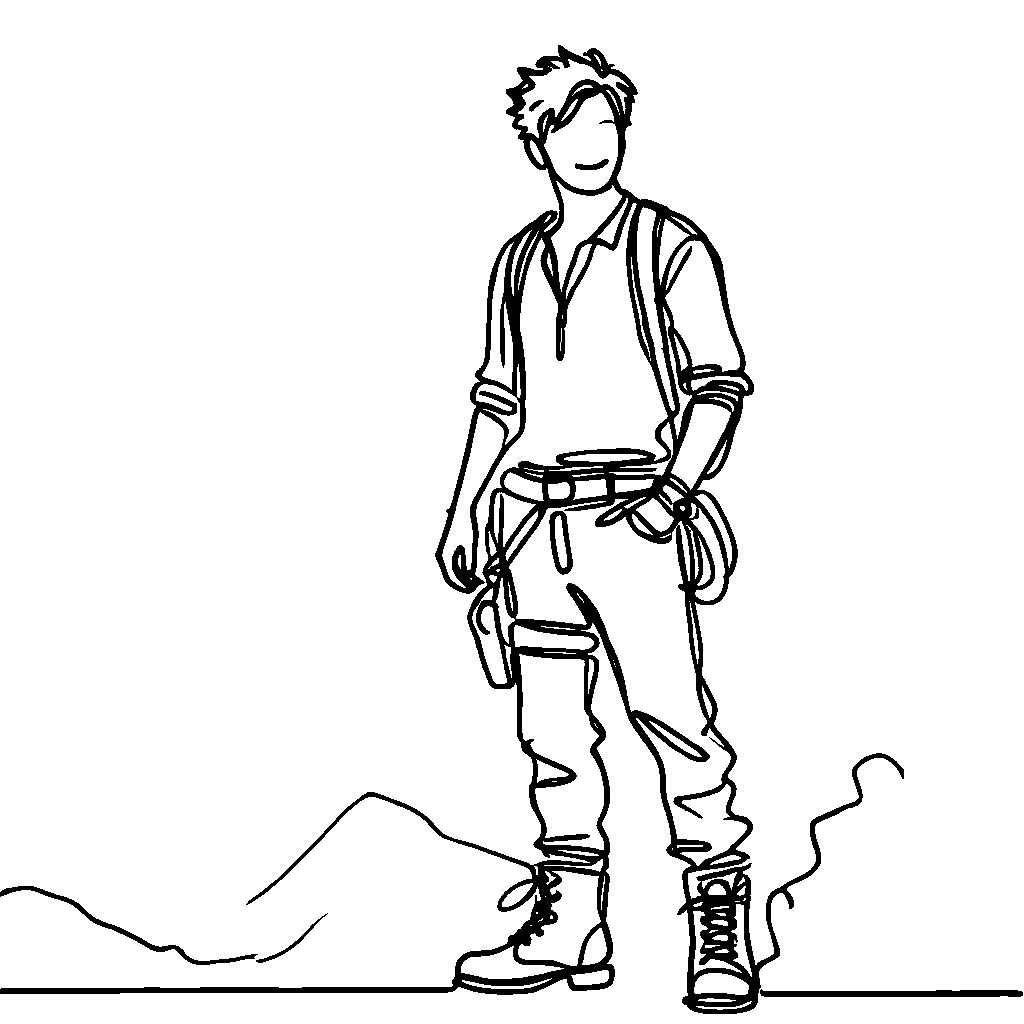
\includegraphics[width=\linewidth]{../presentations/images/lecture_zksnark/urtreasurehunter.jpg}
            \end{column}
    
            \begin{column}{0.7\textwidth}
                Imagine you're part of a treasure hunt...
            \end{column}
        \end{columns}

        \pause

        \begin{columns}
            \begin{column}{0.7\textwidth}
                ...and you've found a hidden treasure chest...
            \end{column}

            \begin{column}{0.2\textwidth}
                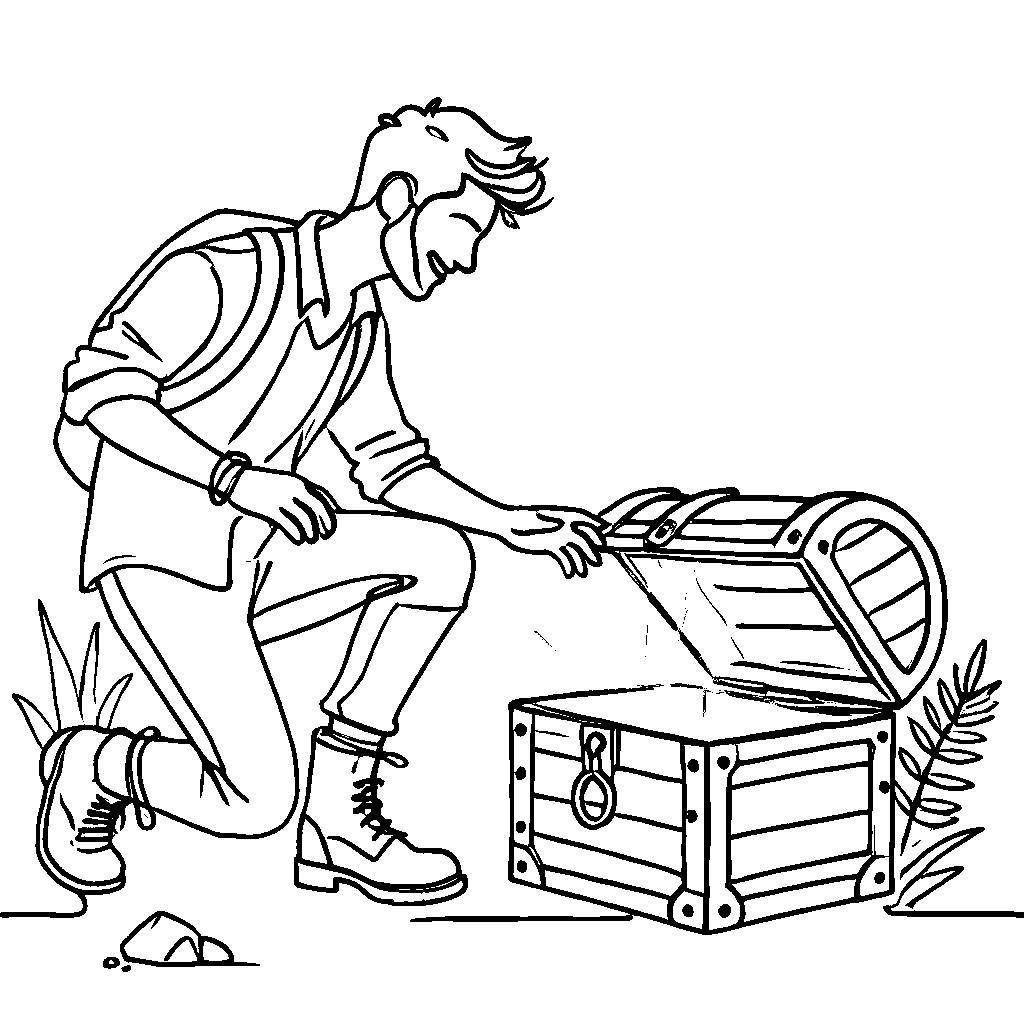
\includegraphics[width=\linewidth]{../presentations/images/lecture_zksnark/uvefoundtreasure.jpg}
            \end{column}
        \end{columns}

        \pause

        \begin{columns}
            \begin{column}{0.2\textwidth}
                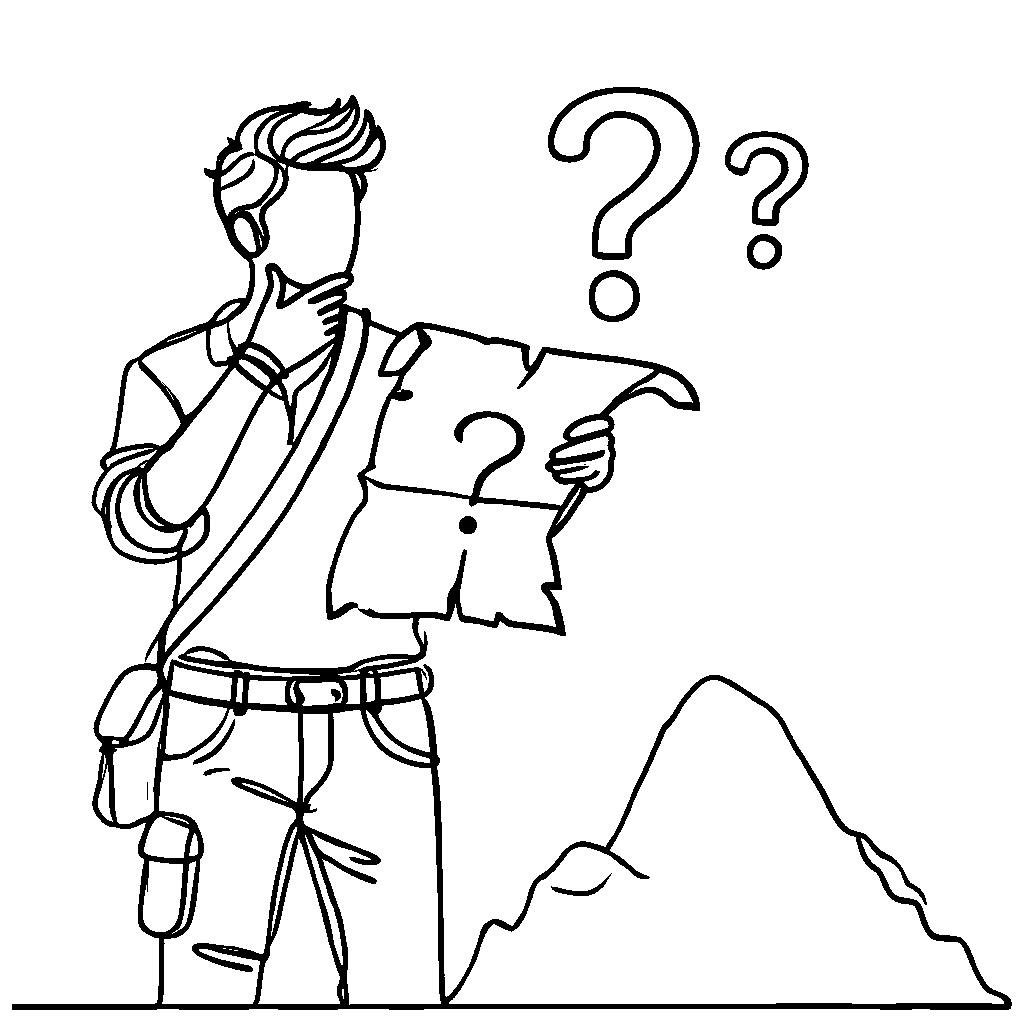
\includegraphics[width=\linewidth]{../presentations/images/lecture_zksnark/howtomakeaproof.jpg}
            \end{column}

            \begin{column}{0.7\textwidth}
                ...but how to prove that without revealing the chest location?
            \end{column}
        \end{columns}
    \end{frame}

    \begin{frame}{Still didn't get who is Snark...}
        \begin{columns}
            \begin{column}{0.65\textwidth}
                \textbf{The Problem}: you have found a hidden treasure chest, and you want to 
                prove to the organizer that you know its location without actually revealing that.
            \end{column}

            \begin{column}{0.3\textwidth}
                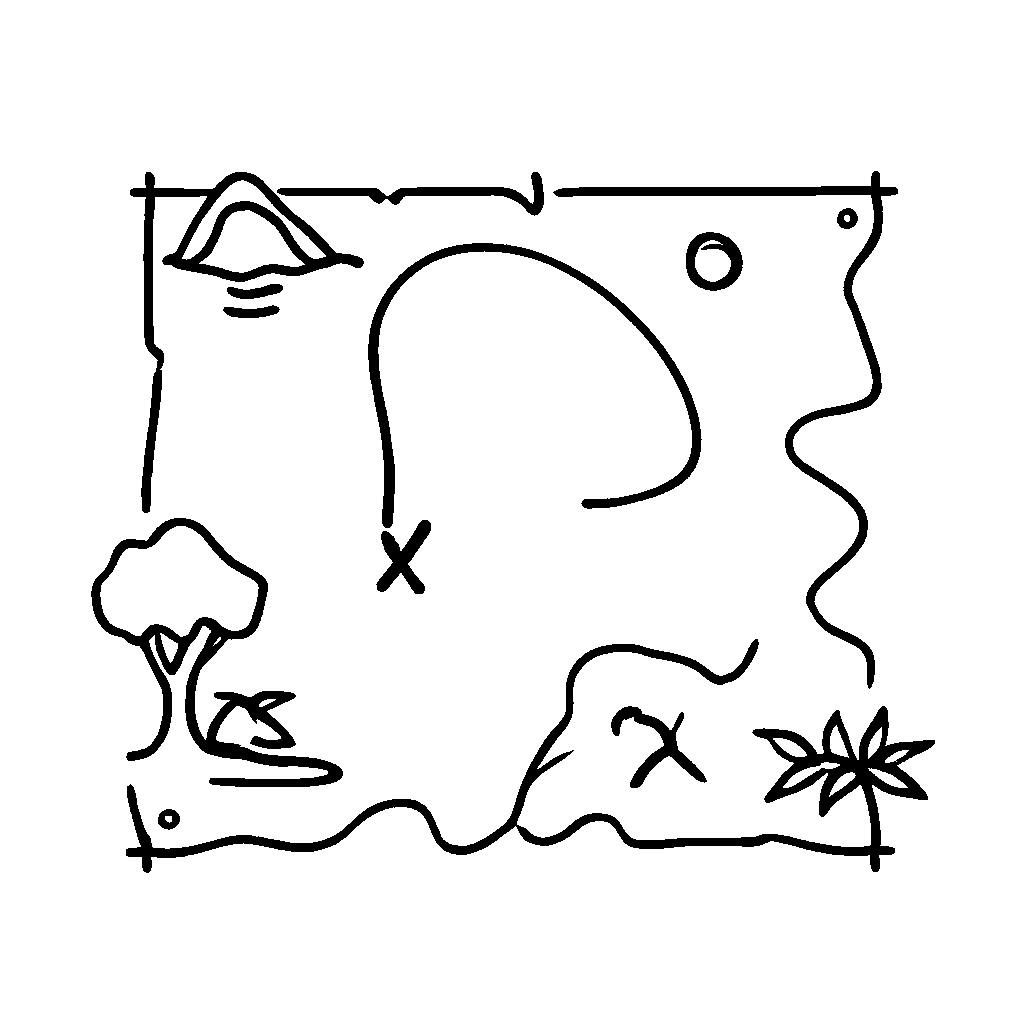
\includegraphics[width=\textwidth]{../presentations/images/lecture_zksnark/treasurelocation.jpg}
            \end{column}
        \end{columns}

        \pause

        We can retrieve some information from that:

        \begin{alertblock}{Question \#81673}
            What is a secret data? Who is a prover and who is a verifier?            
        \end{alertblock}

        \pause

        \vspace{0.1cm}
        \textbf{The Secret Data}: the exact treasure location.

        \vspace{0.1cm}
        \textbf{The Prover}: you.

        \vspace{0.1cm}
        \textbf{The Verifier}: the treasure hunt organizer.
    \end{frame}

    \begin{frame}{Ohh... Got it!}
        Here is how we can apply the zk-SNARK to our problem:

        \begin{itemize}
            \item Argument of Knowledge: You need to create a proof that demonstrates you know the
            chest is.
            \item Succinct: The proof you provide is very small and concise. It doesn't matter how
            large the treasure map is or how many steps it took you to find the chest.
            \item Non-interactive: You don't need to have a back-and-forth conversation with the 
            organizer to create this proof.
            \item Zero-Knowledge: The proof doesn't reveal any information about the actual 
            location of the treasure chest.
        \end{itemize}

        \pause

        \begin{columns}
            \begin{column}{0.3\textwidth}
                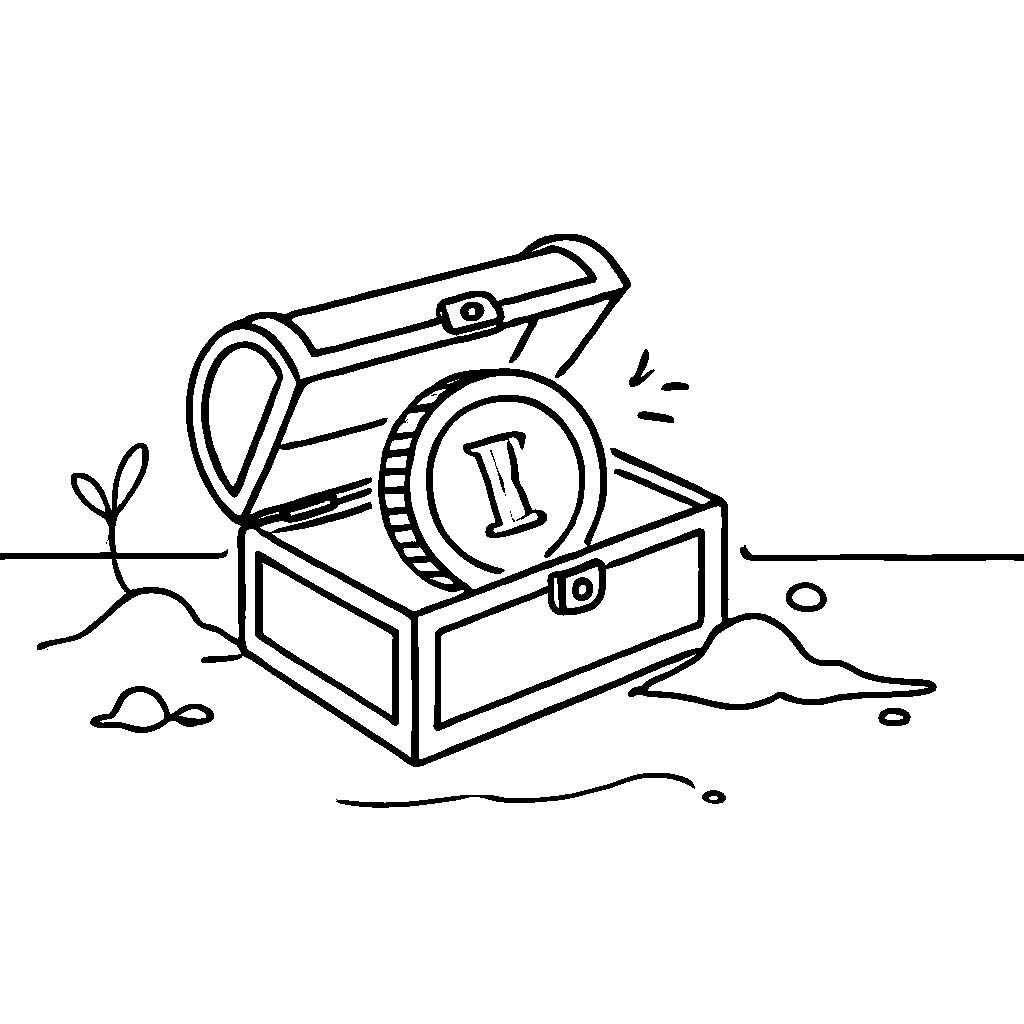
\includegraphics[width=\textwidth]{../presentations/images/lecture_zksnark/treasure.jpg}
            \end{column}

            \begin{column}{0.65\textwidth}
                Well... The golden coin where the pirates' sign is engraved is our zk-SNARK proof!
            \end{column}
        \end{columns}
    \end{frame}

    \begin{frame}
        But the problems that we usually want to solve are in a slightly different format.

        \pause

        \vspace{0.2cm}
        When we need to prove that some element is in a merkle tree, we can't come
        to a verifier and give them a coin...

        \pause

        \center
        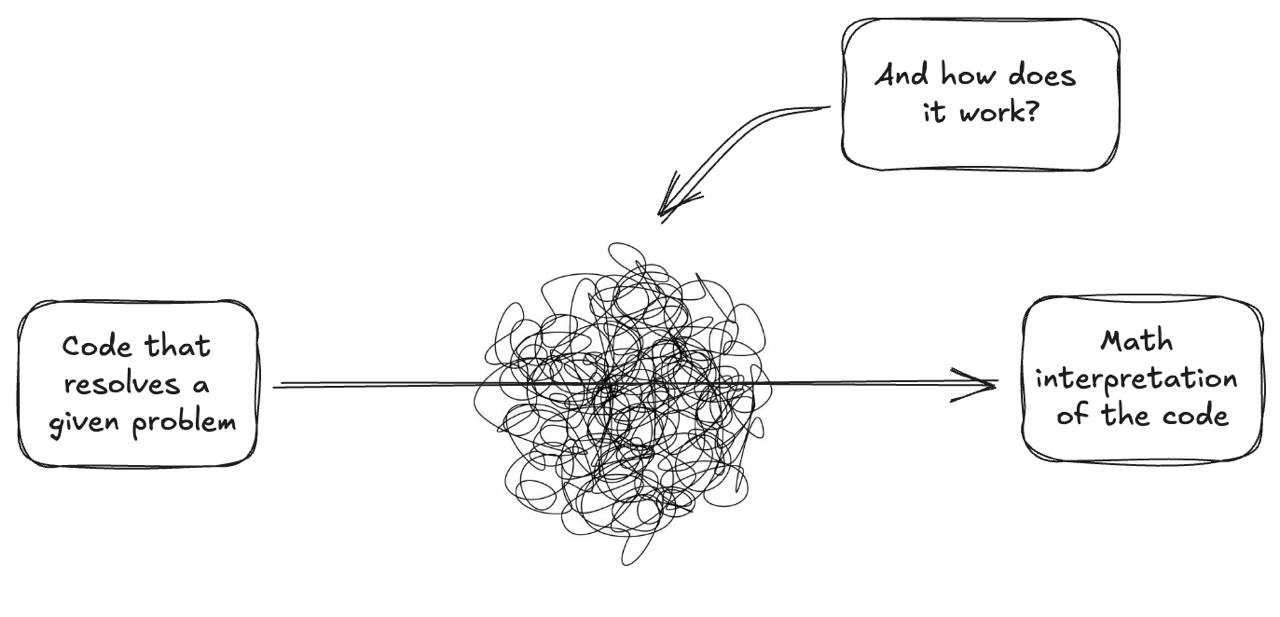
\includegraphics[width=10cm]{../presentations/images/lecture_zksnark/exactcodetomathflow.jpg}
    \end{frame}

    \section{Linear Algebruh Preliminaries}

    \subsection{Inner product}

    \begin{frame}{Inner product}
        TODO
    \end{frame}

    \subsection{Outer product}

    \begin{frame}{Outer product}
        TODO
    \end{frame}

    \section{Arithmetic Circuits}

    \begin{frame}

    \end{frame}

    \section{Rank-1 Constraint System}

    \section{Quadratic Arithmetic Program}
\end{document}